
\begin{figure}[htbp]
\centering
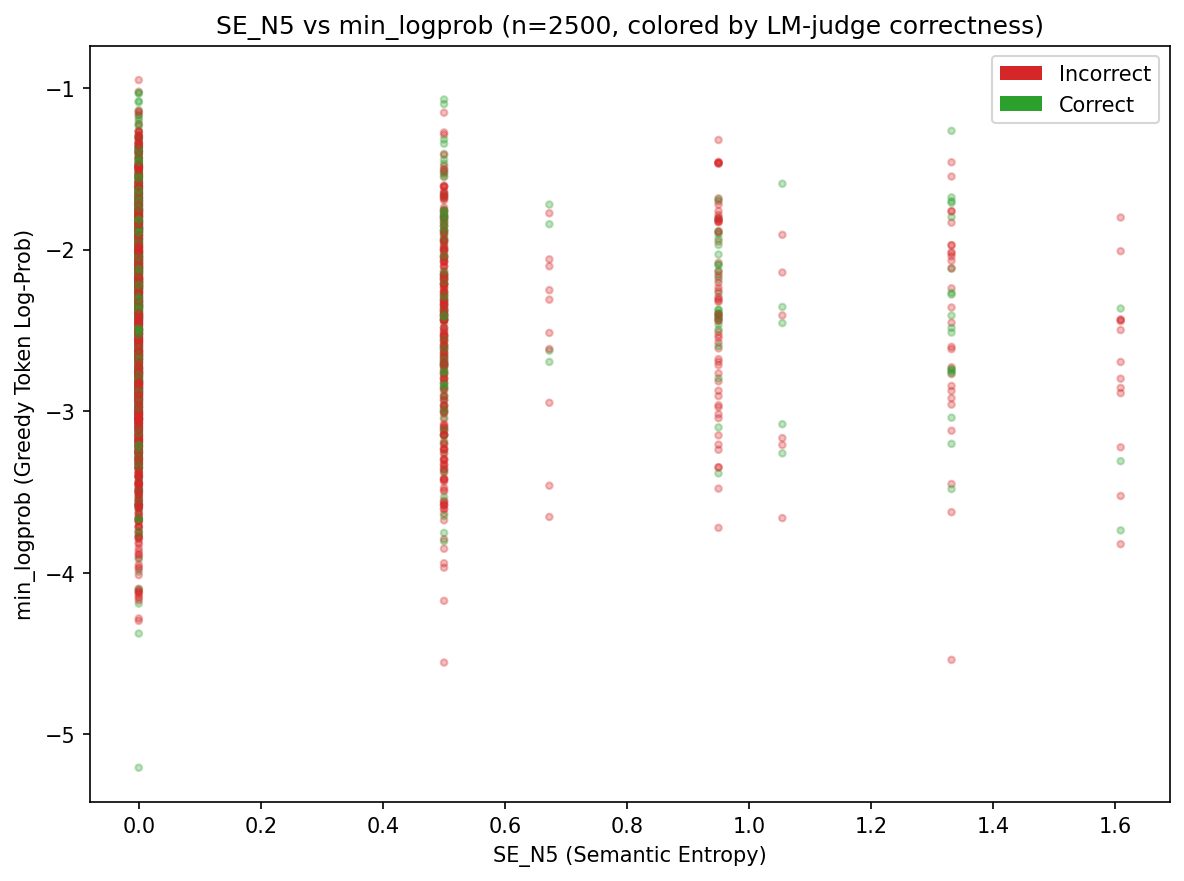
\includegraphics[width=\columnwidth]{figures/scatter_se_vs_minlogprob.png}
\caption{Figure 1: SE\_N5 vs min\_logprob scatter (N=2500), colored by LM-judge correctness}
\label{fig:scatter_se_vs_minlogprob}
\end{figure}

\textit{Figure 1.} SE\_N5 vs. min\_logprob scatter plot (N=2500 prompts), colored by LM-judge correctness (Qwen-2.5-7B). The near-zero linear trend confirms Pearson |r|=0.026. Correctness labels are distributed throughout the joint space without cluster structure indicating signal redundancy.

\begin{figure}[htbp]
\centering
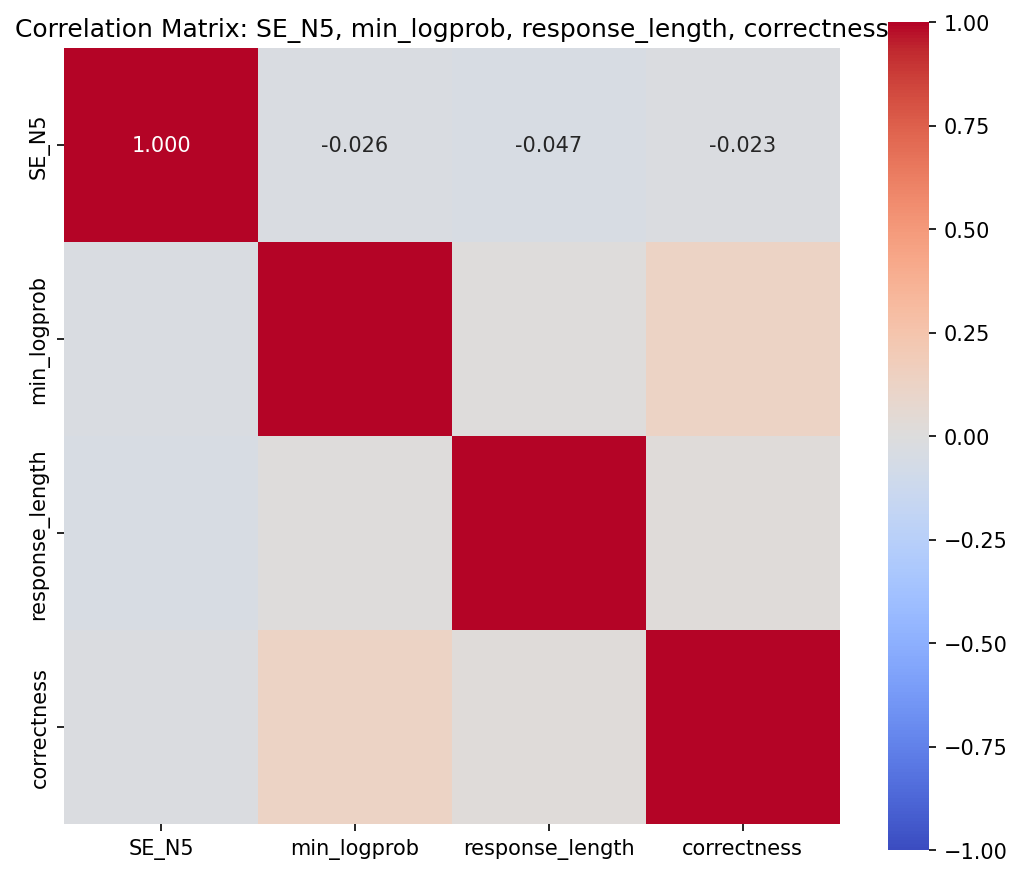
\includegraphics[width=\columnwidth]{figures/correlation_heatmap.png}
\caption{Figure 2: Pearson correlation matrix}
\label{fig:correlation_heatmap}
\end{figure}

\textit{Figure 2.} Pearson correlation matrix for [SE\_N5, min\_logprob, response\_length, correctness]. The near-zero cross-correlation between SE and min\_logprob (|r|=0.026) is visible alongside the moderate individual correlations each signal has with correctness.

\begin{figure}[htbp]
\centering
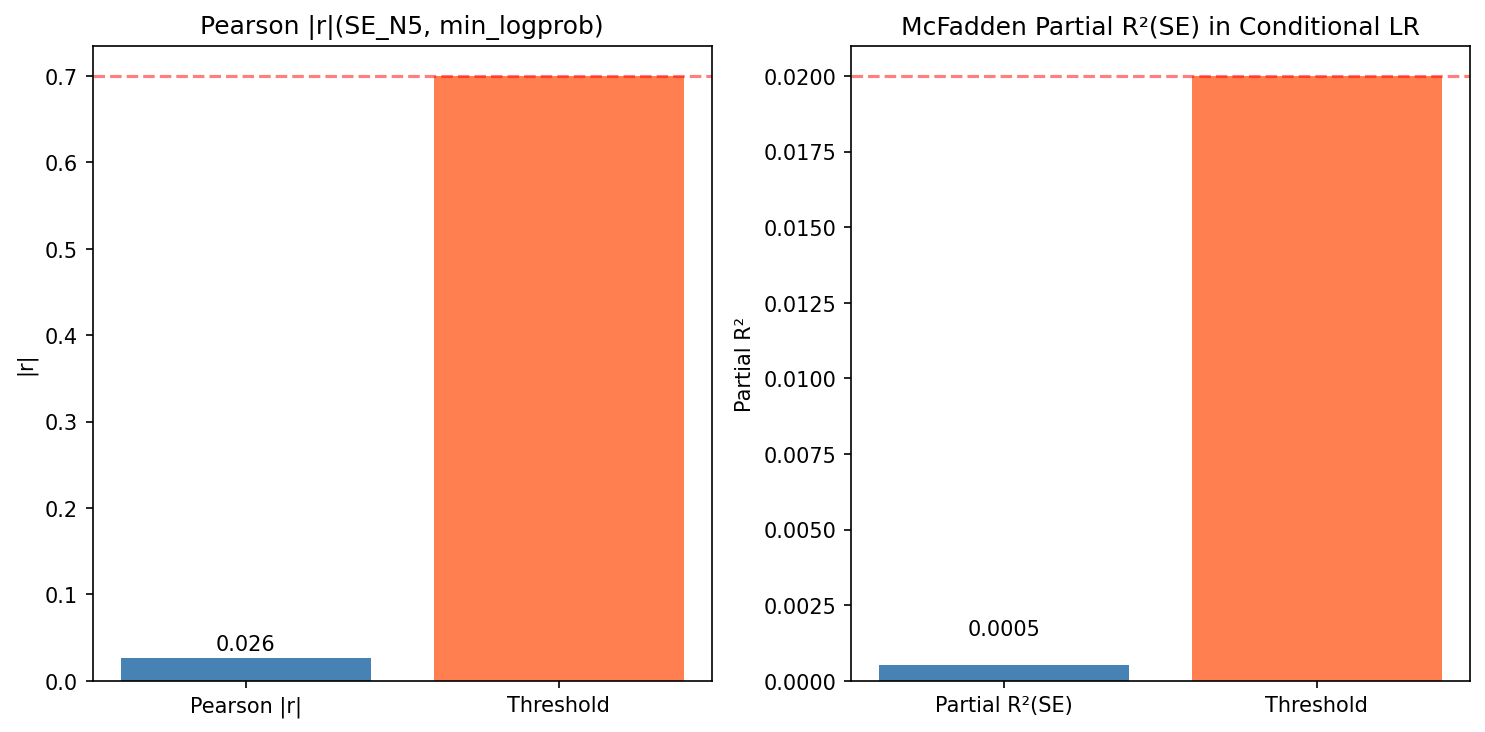
\includegraphics[width=\columnwidth]{figures/gate_metrics.png}
\caption{Figure 3: Gate evaluation bar chart}
\label{fig:gate_metrics}
\end{figure}

\textit{Figure 3.} Gate evaluation: Pearson |r|=0.026 vs. 0.70 threshold (PASS); partial $R^{2}=0.0005$ vs. 0.02 threshold (below threshold; gate outcome EXPLORE\_N10).

\begin{figure}[htbp]
\centering
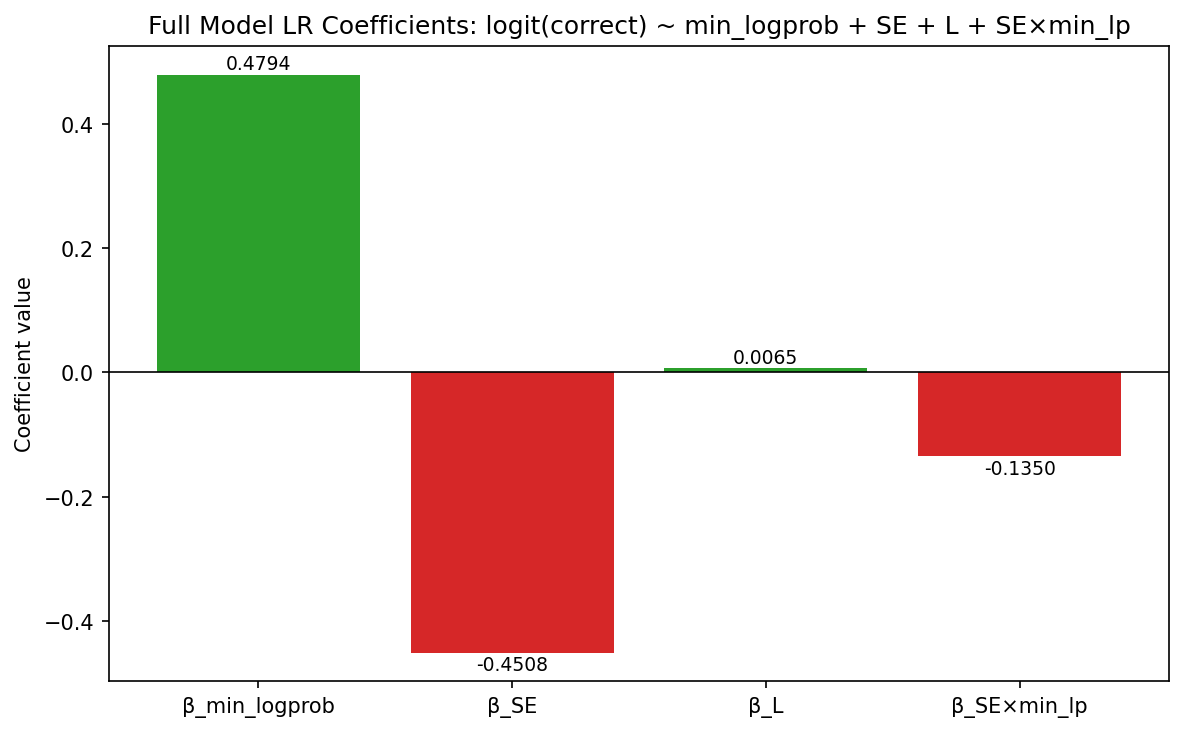
\includegraphics[width=\columnwidth]{figures/lr_coefficients.png}
\caption{Figure 4: Logistic regression coefficients with 95\% CI}
\label{fig:lr_coefficients}
\end{figure}

\textit{Figure 4.} Conditional logistic regression coefficients with 95\% CI for [min\_logprob, SE, L, $SE\times min$\_logprob]. The SE coefficient ($\beta _{2})$ is positive (correct direction) but the confidence interval crosses zero at N=2500, consistent with a powered null result.
